\documentclass[aspectratio=169, 10pt]{beamer}

\usetheme{Madrid}
\usecolortheme{default}
\setbeamertemplate{navigation symbols}{}
\setbeamertemplate{footline}[frame number]

\usepackage{amsmath, amssymb}
\usepackage{booktabs}
\usepackage{graphicx}

\title[RWMH Proposal Scaling]{Random-Walk Metropolis--Hastings:\\How Proposal Scale Affects Mixing and Estimation Accuracy}
\subtitle{MATH 3428 Statistical Computing — Fall 2026--27}
\author[Mai, Siu, Lee]{MAI, Qinyuan (21153159) \and SIU, Tsz Cheung (21174787) \and LEE, Hoi Kiu (21175262)}
\date{November 2026}

\begin{document}

% -------------------------------------------------------------------------
% SLIDE 1: Title & Research Question (0:00 - 0:40)
% -------------------------------------------------------------------------
\begin{frame}
  \titlepage
\end{frame}

% -------------------------------------------------------------------------
% SLIDE 2: Motivation & Classical Theory (0:40 - 1:25)
% -------------------------------------------------------------------------
\begin{frame}{1. Question \& Motivation: The Proposal Scale Trade-Off}
  \textbf{Random-Walk Metropolis--Hastings (RWMH)} proposes moves via:
  \[
    x' = x_t + \sigma \xi, \qquad \xi \sim \mathcal{N}(0, I_d)
  \]
  The single tuning parameter $\sigma > 0$ controls a fundamental trade-off:
  \begin{itemize}
    \item \textbf{$\sigma$ too small:} Almost all proposals accepted, but tiny steps $\implies$ slow random drift.
    \item \textbf{$\sigma$ too large:} Proposals jump into low-density tails $\implies$ high rejection, sticky chain.
  \end{itemize}

  \vspace{0.3em}
  \begin{block}{Classical Optimal-Scaling Theory (Roberts, Gelman \& Gilks, 1997; Roberts \& Rosenthal, 2001)}
    For $d$-dimensional product targets as $d \to \infty$:
    \begin{itemize}
      \item Optimal proposal scale: $\displaystyle \sigma^\star = \frac{2.38}{\sqrt{d}}$
      \item Asymptotic optimal acceptance rate: $\approx \mathbf{0.234}$ \quad (for $d=1$: $\approx \mathbf{0.44}$)
    \end{itemize}
  \end{block}

  \vspace{0.2em}
  \textbf{Project Question:} How does $\sigma$ affect mixing and estimation accuracy, and when does the $\sigma^\star = 2.38/\sqrt{d}$ ($0.234$) rule hold or break down across dimensions, budgets, and correlations?
\end{frame}

% -------------------------------------------------------------------------
% SLIDE 3: Algorithm & Practical Implementation (1:25 - 2:15)
% -------------------------------------------------------------------------
\begin{frame}{2. Method \& Self-Implemented Architecture}
  \begin{columns}[T]
    \begin{column}{0.48\textwidth}
      \textbf{RWMH Algorithm (\texttt{code/algorithm.py}):}
      \begin{enumerate}
        \item \textbf{Propose:} $\xi \sim \mathcal{N}(0, I_d)$, $x' = x_t + \sigma\xi$.
        \item \textbf{Log Ratio:} $\log\alpha = \log\pi(x') - \log\pi(x_t)$\\
              \textit{(Symmetric proposal $\implies$ Hastings ratio cancels)}.
        \item \textbf{Accept/Reject:} Draw $U \sim \mathrm{Unif}(0,1)$; set $x_{t+1} = x'$ if $\log U < \log\alpha$, else $x_{t+1} = x_t$.
      \end{enumerate}
      \vspace{0.3em}
      \textbf{Key Numerical Choices:}
      \begin{itemize}
        \item \textbf{Log-scale arithmetic:} Prevents floating-point underflow in high dimensions.
        \item \textbf{Burn-in \& Thinning:} Discard burn-in; keep \texttt{thin = 1} since ESS is more informative.
      \end{itemize}
    \end{column}

    \begin{column}{0.50\textwidth}
      \textbf{Diagnostics (\texttt{code/diagnostics.py}):}
      \begin{itemize}
        \item \textbf{Fast ACF via FFT:} Biased autocovariance $\hat{\gamma}_k$ computed in $\mathcal{O}(N\log N)$ time; returns \texttt{NaN} safely if chain variance is zero (frozen chain).
        \item \textbf{Effective Sample Size (Geyer, 1992):}
        \[
          \widehat{\mathrm{ESS}} = \frac{N}{1 + 2\sum_{k=1}^{K} \hat{\rho}_k}
        \]
        Summing positive autocorrelations until the first lag where $\hat{\rho}_k \le 0$ (initial positive sequence).
        \item \textbf{Independent Replications ($R$ runs):} Directly estimates empirical $\mathrm{MSE}(\hat{\mu}) = \frac{1}{R}\sum_{r=1}^R \|\hat{\mu}^{(r)} - \mu\|^2$ and standard errors.
      \end{itemize}
    \end{column}
  \end{columns}
\end{frame}

% -------------------------------------------------------------------------
% SLIDE 4: Validation (2:15 - 3:05)
% -------------------------------------------------------------------------
\begin{frame}{3. Validation on $\mathcal{N}(0, I_5)$ \& The Autocorrelated KS-Test Trap}
  \textbf{Setup (\texttt{code/validation.py}):} $d=5$, $\sigma^\star = 2.38/\sqrt{5} \approx 1.064$, $N = 200,000$ post-burn-in draws.
  \begin{itemize}
    \item \textbf{Moment checks pass:} All 5 coordinate means within $4\times\mathrm{MCSE}$ of $0$; diagonal variances $\in [1.001, 1.020]$; max off-diagonal $|\hat{\rho}_{jk}| = 0.012$.
    \item \textbf{Why Raw KS Tests Reject ($p < 0.01$):} Standard Kolmogorov--Smirnov assumes i.i.d.\ draws. Positive MCMC autocorrelation inflates the test statistic at $N=200,000$.
    \item \textbf{Fix — Thinning to ESS ($\approx 11,112$ draws, $\text{thin} \approx 18$):} Restores near-independence; 4 of 5 coordinates pass at $\alpha = 0.05$ (1 marginal $p=0.030$ expected under 5 tests).
  \end{itemize}

  \vspace{0.2em}
  \centering
  \footnotesize
  \begin{tabular}{rrrr|rr|rrr}
    \toprule
    & \multicolumn{3}{c|}{\textbf{Moment Recovery ($N=200,000$)}} & \multicolumn{2}{c|}{\textbf{Raw KS Test}} & \multicolumn{3}{c}{\textbf{ESS-Thinned KS Test}} \\
    \textbf{Dim} & \textbf{Mean Est.} & \textbf{MCSE} & \textbf{Var Est.} & \textbf{KS Stat} & \textbf{$p$-val} & \textbf{Thin} & \textbf{KS Stat} & \textbf{$p$-val} \\
    \midrule
    0 & $-0.0132$ & $0.0093$ & $1.0010$ & $0.0080$ & $0.000$ & 18 & $0.0119$ & $0.086$ \\
    1 & $-0.0193$ & $0.0093$ & $1.0016$ & $0.0107$ & $0.000$ & 18 & $0.0088$ & $0.349$ \\
    2 & $+0.0028$ & $0.0091$ & $1.0032$ & $0.0037$ & $0.009$ & 17 & $0.0064$ & $0.722$ \\
    3 & $-0.0169$ & $0.0093$ & $1.0122$ & $0.0079$ & $0.000$ & 18 & $0.0090$ & $0.330$ \\
    4 & $-0.0005$ & $0.0093$ & $1.0199$ & $0.0073$ & $0.000$ & 17 & $0.0133$ & $0.030$ \\
    \bottomrule
  \end{tabular}
\end{frame}

% -------------------------------------------------------------------------
% SLIDE 5: Qualitative Mixing - Trace & ACF (3:05 - 3:55)
% -------------------------------------------------------------------------
\begin{frame}{4. Visualizing Mixing: Trace Plots \& ACF ($d = 5$)}
  \begin{columns}[c]
    \begin{column}{0.54\textwidth}
      \centering
      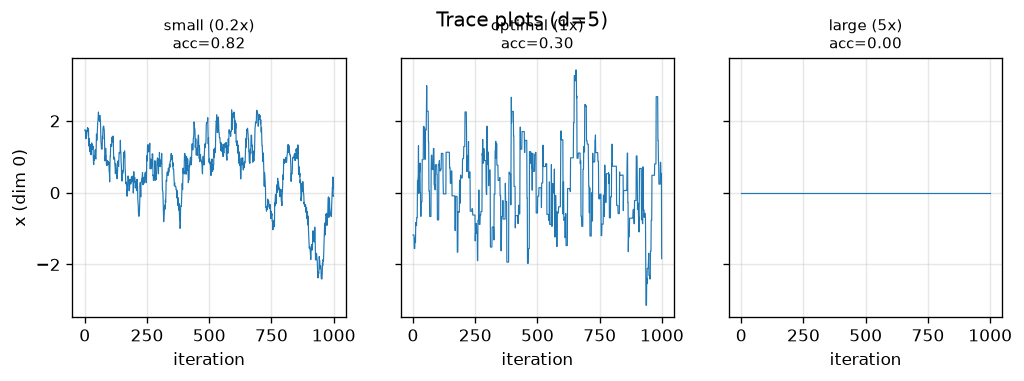
\includegraphics[width=\textwidth]{outputs/figures/fig5_trace.png}
    \end{column}
    \begin{column}{0.44\textwidth}
      \centering
      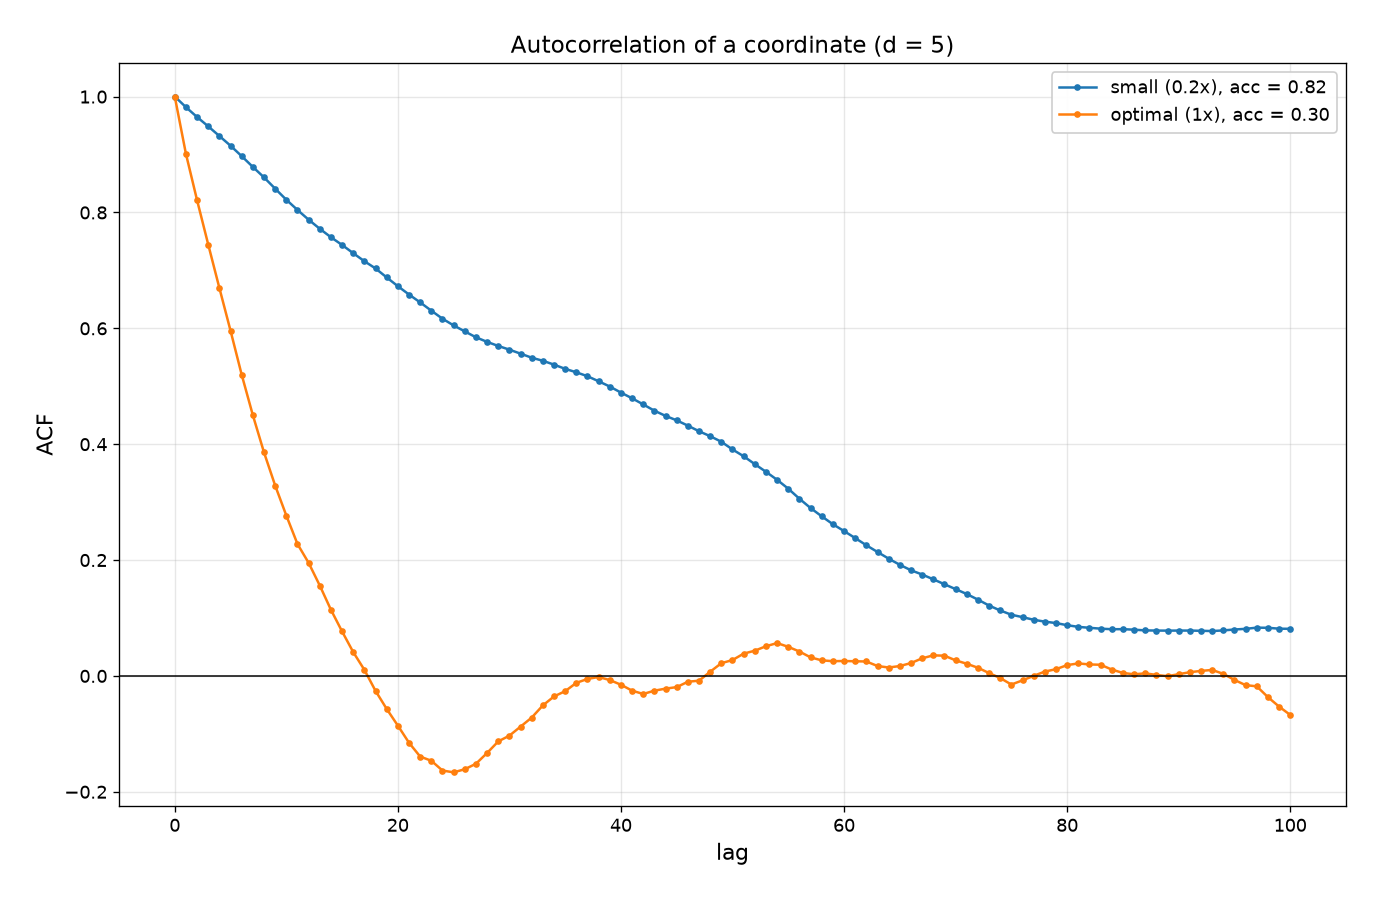
\includegraphics[width=\textwidth]{outputs/figures/fig6_acf.png}
    \end{column}
  \end{columns}
  \vspace{0.3em}
  \begin{itemize}
    \item \textbf{Too small ($0.2\sigma^\star$, acc $= 0.89$):} Slow random-walk drift; ACF stays high for $>100$ lags.
    \item \textbf{Optimal ($1.0\sigma^\star$, acc $= 0.30$):} Rapid stationary mixing; ACF decays to zero by lag $\approx 20$.
    \item \textbf{Too large ($5.0\sigma^\star$, acc $= 0.00$):} Zero accepted moves in $1,000$ steps! Chain stays frozen at $x_0 = 0$ (zero variance $\implies$ ACF is undefined/omitted).
  \end{itemize}
\end{frame}

% -------------------------------------------------------------------------
% SLIDE 6: Main Scaling Study - Acceptance & MSE vs Scale (3:55 - 4:55)
% -------------------------------------------------------------------------
\begin{frame}{5. Main Study: Acceptance Rate \& MSE vs.\ Proposal Scale}
  \textbf{Design:} $d \in \{1, 5, 20\}$, 12 log-spaced scales $\in [0.15\sigma^\star, 8\sigma^\star]$, $N=1500$ (burn-in $500$), $R=100$ reps.
  \begin{columns}[c]
    \begin{column}{0.48\textwidth}
      \centering
      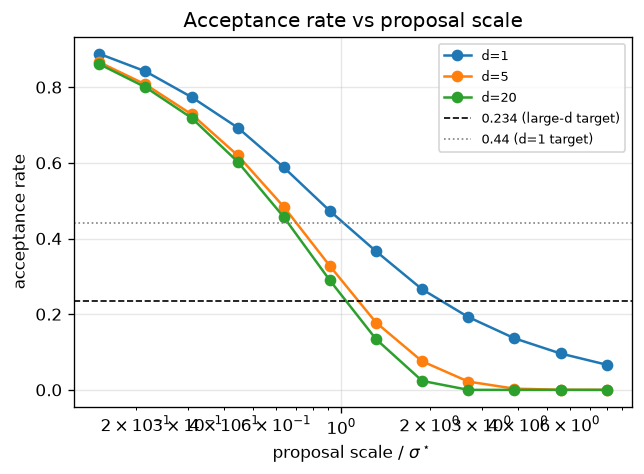
\includegraphics[width=0.95\textwidth]{outputs/figures/fig1_acc_vs_scale.png}
    \end{column}
    \begin{column}{0.48\textwidth}
      \centering
      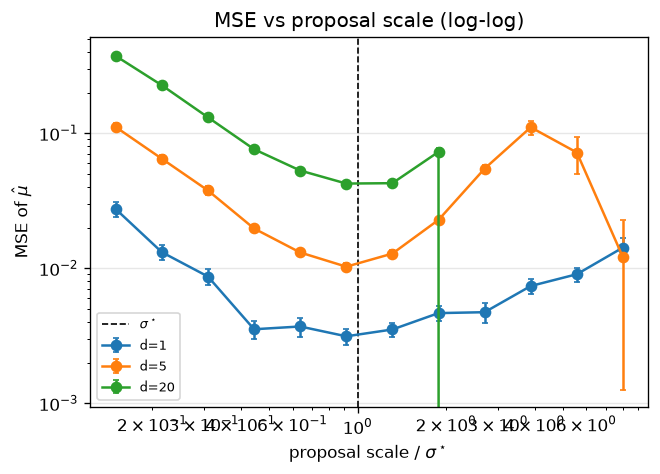
\includegraphics[width=0.95\textwidth]{outputs/figures/fig2_mse_vs_scale.png}
    \end{column}
  \end{columns}
  \begin{itemize}
    \item \textbf{Left (Fig 1):} At $\sigma = \sigma^\star$, acceptance hits $\mathbf{0.446}$ ($d=1$), $\mathbf{0.288}$ ($d=5$), and $\mathbf{0.248}$ ($d=20$), converging toward the theoretical $0.234$ asymptote.
    \item \textbf{Right (Fig 2):} Empirical MSE is U-shaped on log-log axes, minimised near $\sigma / \sigma^\star = 1$.
  \end{itemize}
\end{frame}

% -------------------------------------------------------------------------
% SLIDE 7: MSE vs Acceptance & ESS vs Scale (4:55 - 5:50)
% -------------------------------------------------------------------------
\begin{frame}{6. Tuning by Acceptance Rate \& Effective Sample Size}
  \begin{columns}[c]
    \begin{column}{0.48\textwidth}
      \centering
      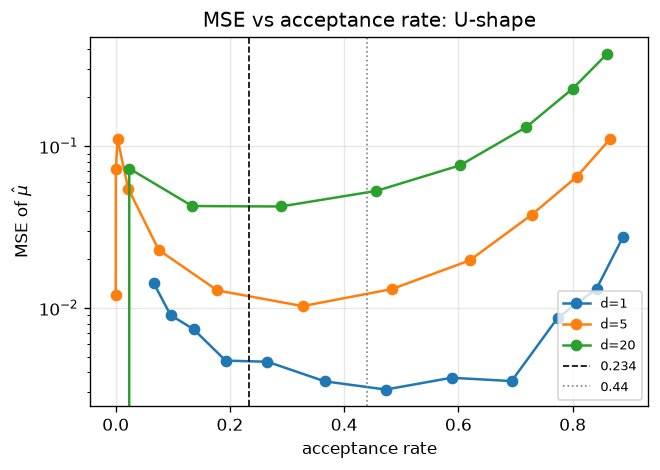
\includegraphics[width=0.95\textwidth]{outputs/figures/fig3_mse_vs_accept.png}
    \end{column}
    \begin{column}{0.48\textwidth}
      \centering
      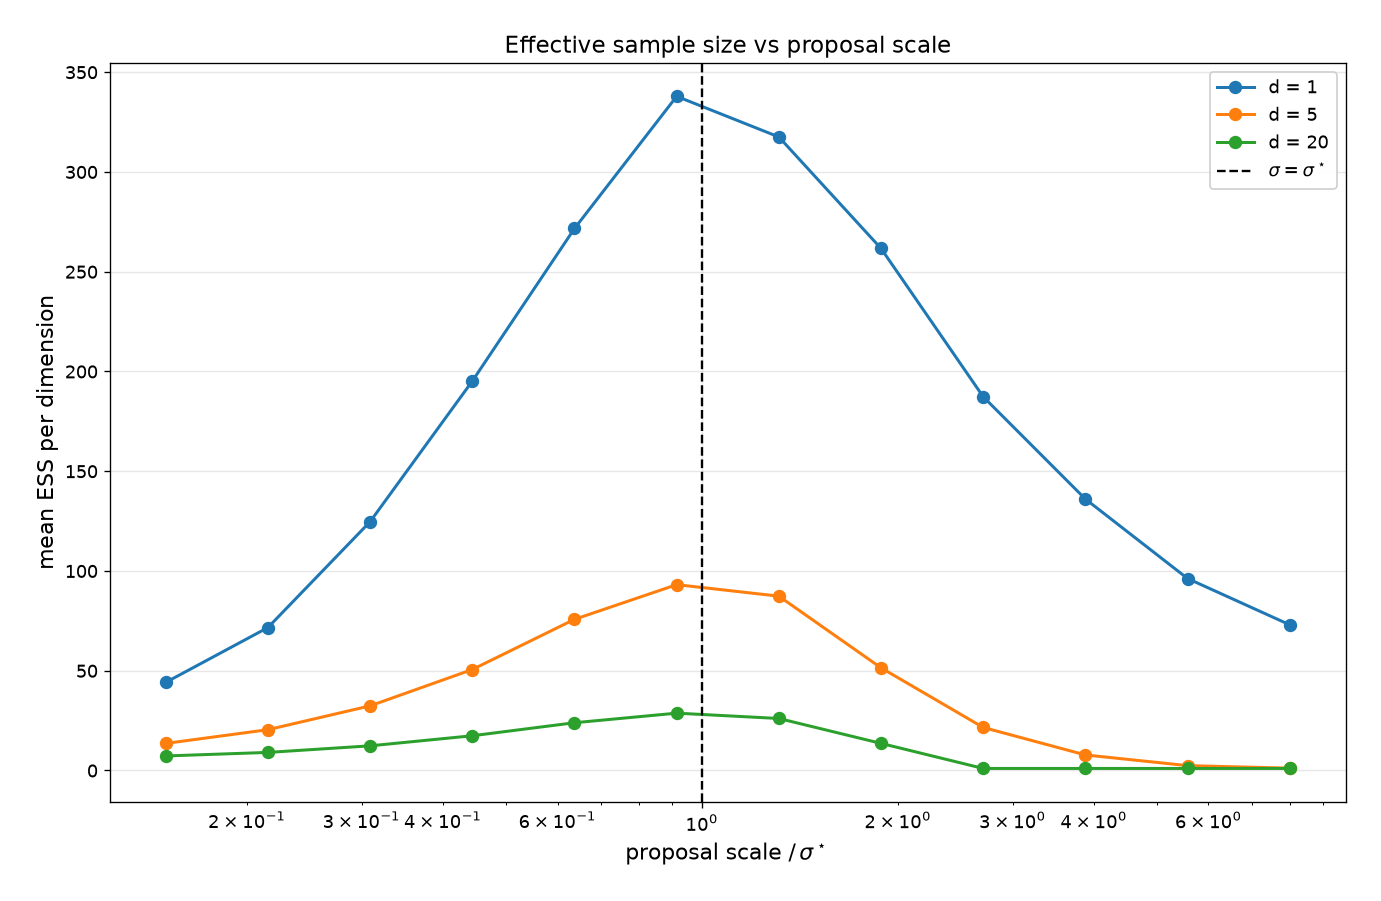
\includegraphics[width=0.95\textwidth]{outputs/figures/fig4_ess_vs_scale.png}
    \end{column}
  \end{columns}
  \vspace{0.2em}
  \centering
  \footnotesize
  \begin{tabular}{rrrrr}
    \toprule
    \textbf{Dim $d$} & \textbf{Ref.\ Scale $\sigma^\star = 2.38/\sqrt{d}$} & \textbf{Acc.\ at $\sigma^\star$} & \textbf{$\mathrm{ESS}/N$ at $\sigma^\star$} & \textbf{MSE at $\sigma^\star$} \\
    \midrule
    1  & $2.380$ & $0.446$ & $0.230$ & $2.49 \times 10^{-3}$ \\
    5  & $1.064$ & $0.288$ & $0.062$ & $1.16 \times 10^{-2}$ \\
    20 & $0.532$ & $0.248$ & $0.019$ & $3.90 \times 10^{-2}$ \\
    \bottomrule
  \end{tabular}
  \begin{itemize}
    \item \textbf{Dimension-dependent optimum (Fig 3):} MSE minimum shifts from $\approx 0.44$ ($d=1$) to $\approx 0.234$ ($d=20$).
    \item \textbf{ESS mirrors MSE (Fig 4):} $\mathrm{ESS}/N$ peaks at $\sigma^\star$ and falls as $\mathcal{O}(1/d)$.
  \end{itemize}
\end{frame}

% -------------------------------------------------------------------------
% SLIDE 8: Baseline Comparison & Budget Scaling (5:50 - 6:45)
% -------------------------------------------------------------------------
\begin{frame}{7. Baseline Comparison (vs.\ i.i.d.) \& Computational Budget}
  \begin{columns}[c]
    \begin{column}{0.52\textwidth}
      \centering
      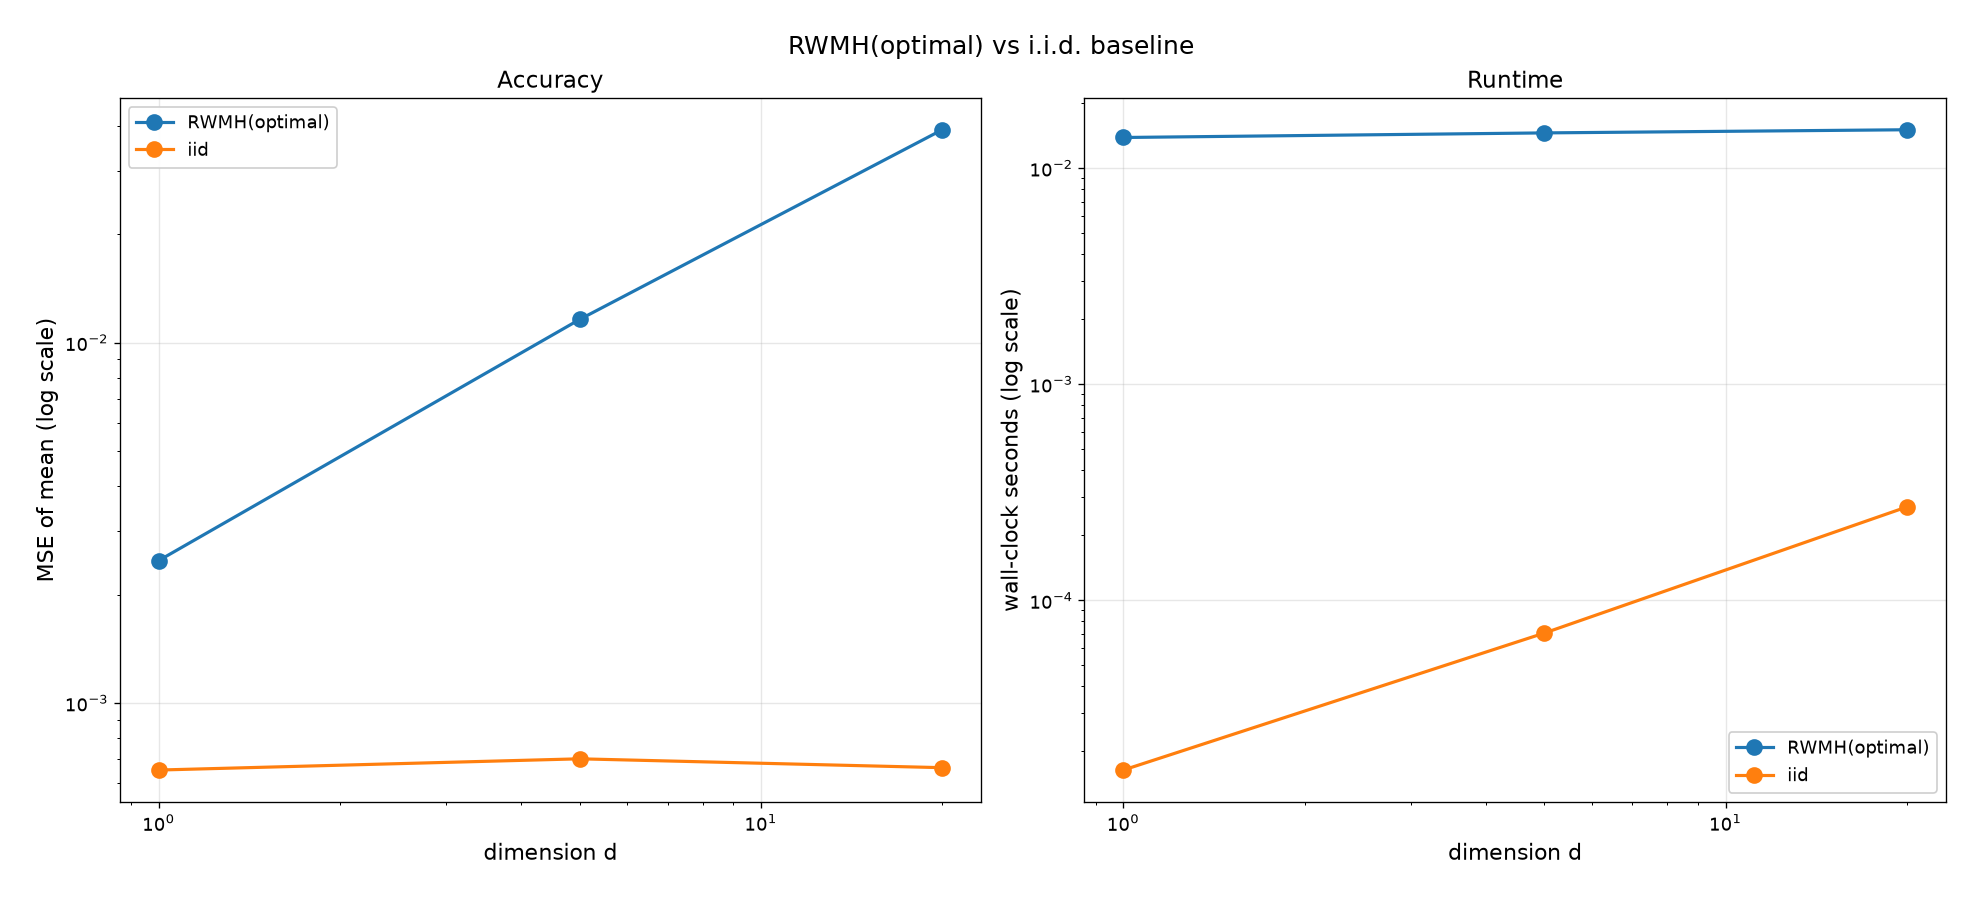
\includegraphics[width=\textwidth]{outputs/figures/fig8_baseline.png}
    \end{column}
    \begin{column}{0.46\textwidth}
      \centering
      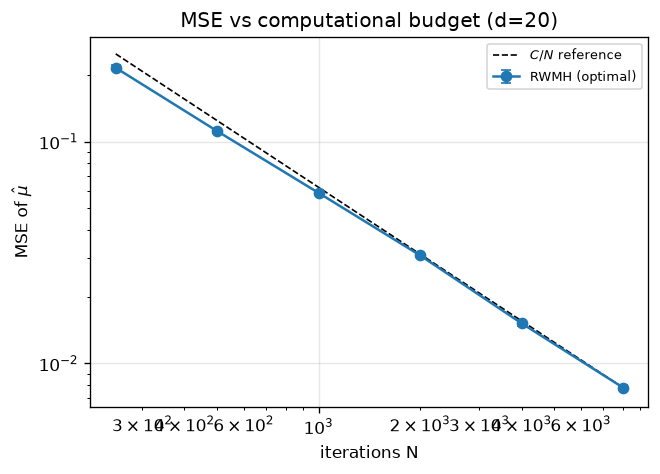
\includegraphics[width=0.95\textwidth]{outputs/figures/fig7_budget.png}
    \end{column}
  \end{columns}
  \vspace{0.2em}
  \begin{itemize}
    \item \textbf{The ``Applicability Tax'' vs.\ i.i.d.\ (Fig 8, $R=200$):} At $N=1500$, optimal RWMH has $\mathbf{3.8\times}$ ($d=1$), $\mathbf{16.6\times}$ ($d=5$), and $\mathbf{59\times}$ ($d=20$) higher MSE than i.i.d.\ sampling, and runs $58\times\text{--}828\times$ slower.
    \item \textbf{Computational Budget Scaling (Fig 7, $d=20$):} Varying $N \in \{250, \dots, 8000\}$ confirms the Markov Chain CLT rate $\mathrm{MSE}(\hat{\mu}) \approx 62.3 / N$ (log-log slope $-1$).
  \end{itemize}
\end{frame}

% -------------------------------------------------------------------------
% SLIDE 9: Robustness Check - Correlated Target (6:45 - 7:25)
% -------------------------------------------------------------------------
\begin{frame}{8. When Classical Scaling Breaks Down: Correlated Targets}
  \begin{columns}[c]
    \begin{column}{0.50\textwidth}
      \centering
      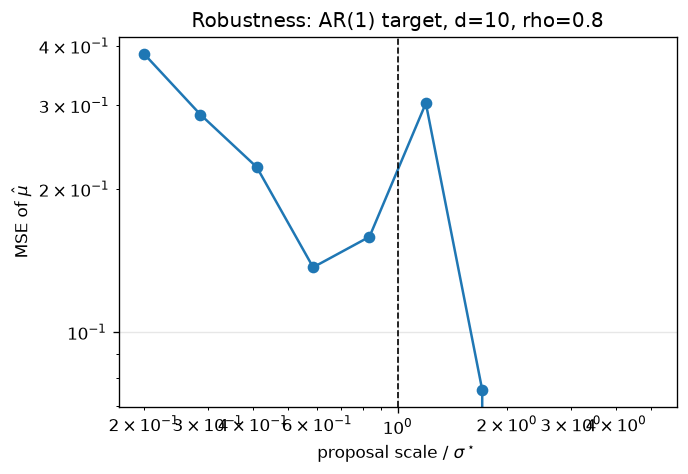
\includegraphics[width=\textwidth]{outputs/figures/fig9_robust_corr.png}
    \end{column}
    \begin{column}{0.48\textwidth}
      \textbf{AR(1) Target ($d=10$, $\Sigma_{jk} = 0.8^{|j-k|}$):}
      \begin{itemize}
        \item Classical $\sigma^\star = 2.38/\sqrt{d}$ assumes the proposal covariance matches the target covariance shape.
        \item Using an \textbf{isotropic} proposal ($\sigma^2 I_d$) on a correlated target flattens the MSE curve and shifts the empirical optimum \textbf{to the right of $\sigma^\star$}.
        \item \textbf{Practical Lesson:} When coordinates are correlated or badly scaled, precondition with an estimated target covariance $\hat{\Sigma} = L L^\top$ ($x' = x_t + \sigma L \xi$) or use adaptive MCMC.
      \end{itemize}
    \end{column}
  \end{columns}
\end{frame}

% -------------------------------------------------------------------------
% SLIDE 10: Critical Analysis & Conclusions (7:25 - 8:00)
% -------------------------------------------------------------------------
\begin{frame}{9. Critical Analysis, Trade-Offs \& Conclusions}
  \begin{block}{Key Takeaways from Our Investigation}
    \begin{enumerate}
      \item \textbf{Asymptotic theory works in moderate $d$:} For well-scaled targets in $d \ge 5$, $\sigma^\star = 2.38/\sqrt{d}$ (acceptance $\approx 0.234$) achieves near-minimal MSE and maximal ESS without manual grid search.
      \item \textbf{Do not force $0.234$ in low dimensions:} In $d=1$, the optimal acceptance rate is $\approx 0.44$; forcing $0.234$ over-scales the proposal and increases rejections.
      \item \textbf{Judge mixing by ESS, not acceptance alone:} Correlated targets ($\rho=0.8$) distort isotropic scaling; ESS and pilot runs diagnose poor geometry directly.
      \item \textbf{Efficiency vs.\ Applicability Trade-Off:} RWMH incurs an $\mathcal{O}(d)$ statistical efficiency penalty relative to i.i.d.\ sampling ($3.8\times$ to $59\times$ higher MSE), motivating preconditioning in medium $d$ and gradient-based MCMC (MALA/HMC) in high $d$.
    \end{enumerate}
  \end{block}

  \vspace{0.3em}
  \centering
  \textbf{Thank you! Questions welcome.}
\end{frame}

\end{document}